\documentclass[letterpaper,12pt]{article}
\usepackage[latin1]{inputenc}
\usepackage{amsmath}
\usepackage{graphicx}

\oddsidemargin  0.3in \evensidemargin 0.3in
\textwidth      5.8in \textheight     8.5in
\topmargin      0in
\parindent      0em     % Indentacion
\parskip        2ex     % Salto entre parrafos

\begin{document}
\pagestyle{empty}
\thispagestyle{empty}

\noindent

\begin{tabular}{lcl}
Tuckey: 
&
 \begin{minipage}{5cm}
  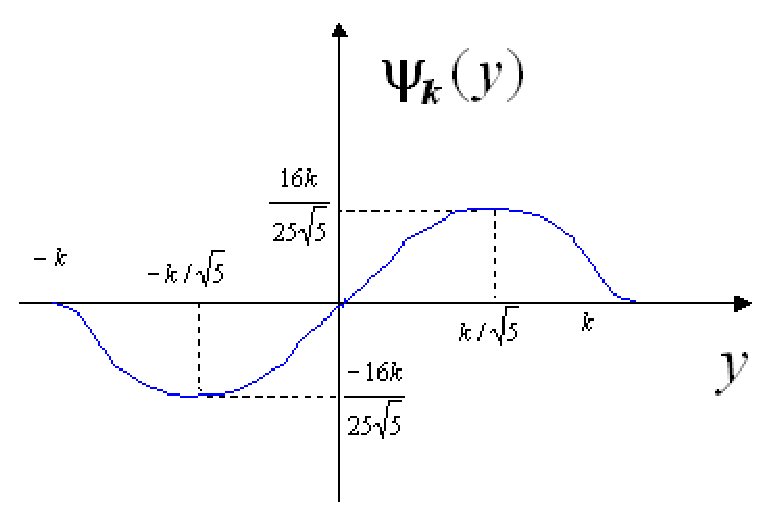
\includegraphics[clip,width=5cm]{tuckey.eps}
 \end{minipage}
&
 \begin{minipage}{6.3cm}
  \begin{equation}
   \psi_k(y) =
   \begin{cases}
    y \Big(1- \big(\frac{y}{k}\big)^2 \Big)^2 & \text{$|y| \le k$} \\
    0 & \text{$|y| > k$}
   \end{cases}
  \end{equation}
 \end{minipage}
\end{tabular}

\end{document}
